\chapter{Medical and Technical Concepts}

\section{Introduction}
This chapter provides essential background information on the clinical and technological context of the thesis. We begin by describing the brain and its tissues from both macroscopic and microscopic perspectives. We then discuss brain tumors, which are the primary focus of this research. Next, we introduce the different types of medical imaging modalities and explain the importance of segmentation tasks in neuro-oncology. Finally, we delve deeper into the principles and components of Magnetic Resonance Imaging (MRI), which is the primary imaging modality used in this thesis.

\section{The Microscopic Description of the Brain}

% \subsection{Macroscopic Description}
The human brain is an irregular, ovoid organ with a large anteroposterior axis. Its average volume is approximately 1100\,cm\textsuperscript{3} in women and 1400\,cm\textsuperscript{3} in men, and it weighs between 1400\,g and 1800\,g. It occupies the cranial cavity but does not contact the bone directly, as it is suspended in cerebrospinal fluid inside a fluid chamber \cite{ref3}.

The brain comprises four main regions: the cerebrum, cerebellum, brainstem, and diencephalon (Figure~\ref{fig:brain-regions}).

\begin{figure}[ht]
  \centering
  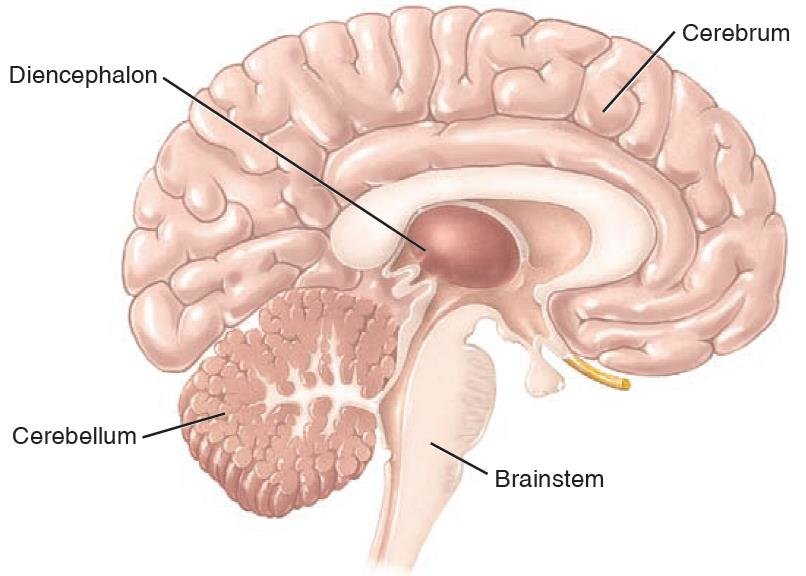
\includegraphics[width=0.5\textwidth]{Images/Chapter0/brain.jpg}
  \caption{Brain main parts: cerebrum, cerebellum, brainstem, and diencephalon \cite{freudenrich2013visualizing}.}
  \label{fig:brain-regions}
\end{figure}

\subsubsection*{Cerebrum}
The cerebrum is the largest part of the brain, representing about 83\% of its total volume. It is divided into right and left hemispheres connected by the corpus callosum. Each hemisphere controls the contralateral side of the body.

% \begin{figure}[ht]
%   \centering
%   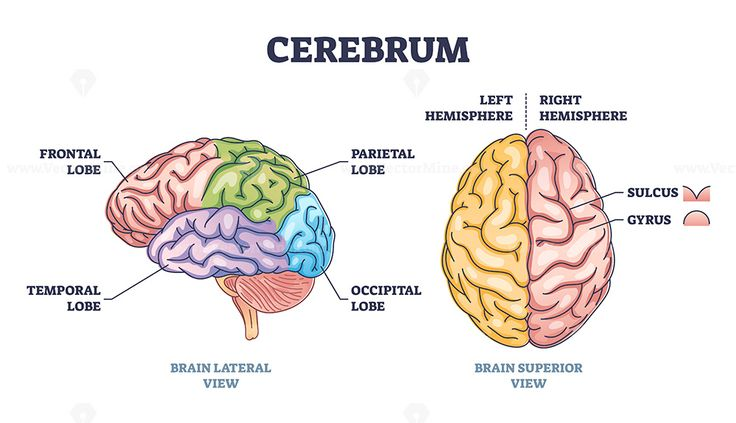
\includegraphics[width=0.7\textwidth]{Images/Chapter0/cerebrum.jpg}
%   \caption{Cerebrum brain structure from lateral and superior view outline diagram \cite{freudenrich2013visualizing}.}
%   \label{fig:cerebrum}
% \end{figure}

% Each hemisphere contains four lobes—frontal, parietal, occipital, and temporal—with distinct functions (Figure~\ref{fig:cerebrum}).



% \paragraph{Frontal lobes}
% \begin{itemize}
%   \item Speech, language, reasoning, decision-making, personality, judgment, and voluntary movements.
%   \item Right frontal lobe controls left-side movements; left frontal lobe controls right-side movements.
% \end{itemize}

% \paragraph{Parietal lobes}
% \begin{itemize}
%   \item Reading, spatial and visual perception, touch, pain, and temperature sensation.
%   \item Right parietal lobe mediates left-side sensitivity; left parietal lobe mediates right-side sensitivity.
% \end{itemize}

% \paragraph{Occipital lobes}
% \begin{itemize}
%   \item Visual processing (color, light, movement).
% \end{itemize}

% \paragraph{Temporal lobes}
% \begin{itemize}
%   \item Language comprehension, memory, and emotion processing.
%   \item Sequencing and organization.
% \end{itemize}

\subsubsection*{Cerebellum}
The cerebellum lies below the cerebrum and accounts for about 11\% of brain volume. It coordinates reflexes, movement, balance, and posture.

\subsubsection*{Brainstem}
The brainstem connects the cerebrum and cerebellum to the spinal cord and controls vital functions such as eye movements, breathing, blood pressure, and heart rate.

\subsubsection*{Diencephalon}
Surrounded by the cerebral hemispheres, the diencephalon coordinates motor functions, maintains consciousness, regulates autonomic functions (eating, thirst, temperature, circadian rhythm) and interacts with both brain and cerebellum \cite{ref4}.
% \subsection{Microscopic Description}
% From a microscopic point of view, the nervous tissue consists of nerve
% cells (neurons) and glial cells (support and protective cells) that derive
% from the ectoderm. Vessels and meninges do not belong to the nervous
% tissue and are derived from the mesoderm.
% The neuron is the cell that constitutes the functional unit of the
% neuroaxis. Neurons are 10 to 50 times more numerous than glial cells.
% The human nervous system comprises about 100 billion neurons. Neurons
% transmit a signal or what we call nerve impulses \cite{ref3}.

\section{Brain Tissue}
The brain's anatomical structures can be divided into hemispheres and lobes, but in medical imaging, voxels are typically classified into three main tissue types: gray matter, white matter, and cerebrospinal fluid (CSF) \cite{ref1}.

\subsection*{Gray Matter}
Gray matter contains neuronal cell bodies (soma), axon tracts, glial cells, capillary blood vessels, and neuropil (dendrites, unmyelinated axons, glia) \cite{ref5}.

\subsection*{White Matter}
White matter consists primarily of myelinated axons (tracts), oligodendrocytes, and astrocytes, forming the brain’s long-range connections \cite{ref5}.

\subsection*{Cerebrospinal Fluid}
Cerebrospinal fluid (CSF) cushions the brain and spinal cord, removes metabolic waste, and maintains proper central nervous system function \cite{ref6}.

\begin{figure}[ht]
  \centering
  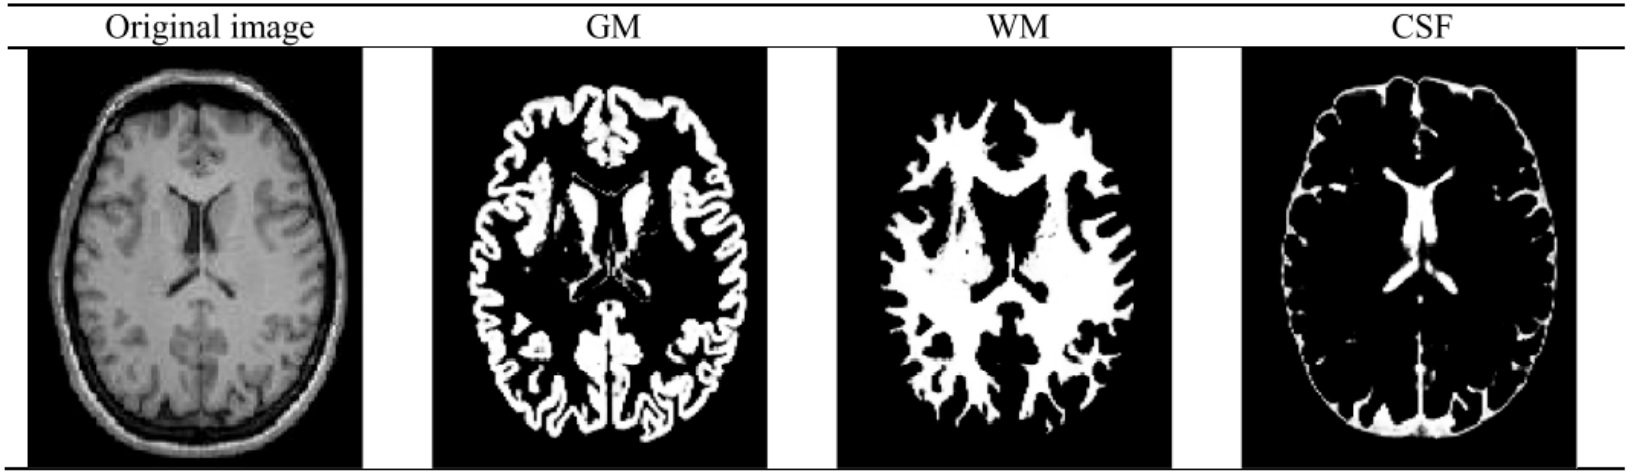
\includegraphics[width=0.7\textwidth]{Images/Chapter0/parts.png}
  \caption{Segmentation of a brain MRI into gray matter (GM), white matter (WM), and CSF by Statistical Parametric Mapping (SPM) \cite{ref7}.}
  \label{fig:spm-segmentation}
\end{figure}

\section{Classification of Brain Tumors}
\label{sec:classification-brain-tumors}

Brain tumors can be categorized by their biological behavior and histology. The World Health Organization (WHO) broadly classifies them as benign, premalignant, or malignant based on growth rate, invasiveness, and cellular atypia \cite{ref8}.

\subsection{Benign Tumors}
Benign tumors grow slowly and do not invade surrounding brain tissue. Histologically, their cells resemble normal counterparts and exhibit low mitotic activity. Common examples include meningiomas and pituitary adenomas, which often present with well‐circumscribed margins and have favorable prognoses following surgical resection \cite{ref8}.

\subsection{Premalignant Tumors}
Premalignant lesions (WHO Grade I–II) display atypical cellular features and proliferative potential higher than benign lesions, yet lack overt invasive behavior. These tumors may progress to higher grades over time, and thus require close monitoring and, in some cases, adjuvant therapy.

\subsection{Malignant Tumors}
Malignant tumors (WHO Grade III–IV) are characterized by rapid growth, high mitotic index, and the ability to infiltrate adjacent neural structures. They often recur despite multimodal treatment (surgery, radiotherapy, chemotherapy) and carry poor overall survival \cite{ref8}.

\section{Common Intracranial Tumor Types}
\label{sec:common-tumor-types}

The three most frequent primary brain tumors in adults are \cite{naser2020lgmi}:

\begin{itemize}
  \item \textbf{Meningioma.}
        Originating from the arachnoidal cap cells of the meninges, meningiomas are typically benign (\glsxtrshort{who} Grade I), slow‐growing, and extra‐axial. They often cause symptoms by mass effect rather than infiltration.

  \item \textbf{Pituitary Adenoma.}
        Arising in the anterior pituitary gland, these adenomas are usually benign but can lead to endocrine dysfunction and visual disturbances due to suprasellar extension.

  \item \textbf{Glioma.}
        Gliomas arise from glial cells and represent the majority of malignant primary \glsxtrshort{cns} tumors. They are graded by WHO as:
        \begin{itemize}
          \item \emph{Low-Grade Glioma (LGG, Grades I–II).} Slow‐growing, with diffuse infiltration but relatively favorable prognosis.
          \item \emph{High-Grade Glioma (HGG, Grades III–IV).} Aggressive, with high proliferative index and poor survival; includes anaplastic astrocytoma (Grade III) and glioblastoma multiforme (Grade IV).
        \end{itemize}
\end{itemize}

Accurate grading of gliomas (LGG vs.\ HGG) is critical for treatment planning and prognosis, and motivates the need for precise segmentation and classification pipelines.


\section{Signs and Symptoms Associated with Brain Tumors}
Brain tumors are the most common cause of death among all people and childhood cancers according to the Surveillance, Epidemiology,
and End Results Program. Signs and symptoms depend on a variety
of factors, including location of the tumor, age of the person, and rate
of tumor growth. Patients with brain tumors develop focal (e.g., motor
deficits, seizures, ocular impairments, urinary incontinence, and speech
impediments) and/or generalized neurological symptoms and signs (e.g.,
headache, nausea, vomiting, dizziness, sleep-wake disturbances, and mentalstatus abnormalities) \cite{ref9}.

\section{Diagnosis of Brain Tumors}
\label{sec:diagnosis-brain-tumors}
The diagnosis of brain tumors is a complex process that requires a combination of clinical evaluation, imaging studies, and sometimes invasive procedures. The following sections outline the key components of this diagnostic process.
\subsection{Physical Examination}
One of the basics of this examination is that the doctor diagnoses the condition of the patient who is under suspicion of a brain tumor, where the doctor studies his condition by interrogating the patient to verify whether there are clinical signs that in turn lead the doctor to do a clinical examination that focuses on functions in which the brain intervenes, such as memory, emotions, understanding the language, feel of touch. By testing these functions, the peripheral symptoms can be detected, and therefore the affected area of the brain.

\subsection{Complementary Examination}
In most cases, the patient's condition requires the doctor to perform various tests, including a lumbar puncture. This is a test in which a sample of the spinal brain fluid is taken by sticking a needle into the lower stem of the spine, with the patient lying on the left side, a needle inserted into the L3 to L4 or L4 to L5. Afterwards, the sample is analyzed to find any cancer cells present for the tumor.

\subsection{Brain Biopsy}
Biopsy is a risky process that can cause bleeding while the surgeon is operating under the patient's total anesthesia, as well as a potential transmission of an infection, whether blood infection or other infection. The goal of this process is to search for cancer and determine its nature by surgically removing a sample of tissues taken from the tumor for closer examination to ascertain the nature of the tissues that are unknown.

\subsection{Medical Imaging}
This examination is based on imaging techniques such as MRI and computed tomography (\glsxtrshort{ct}) scanner or CT scan. MRI was adopted for its unique feature of having detailed, and also it is good technique for knowing the brain tumor in human body, where in the following we will present the general front and characteristics of it \cite{ref10}.


\section{Medical Imaging in Brain Tumor Diagnosis}

Magnetic Resonance Imaging (MRI) has emerged as the gold standard for brain tumor diagnosis due to its superior soft tissue contrast, high spatial resolution, and non-invasive nature. Unlike other imaging modalities such as CT scans, MRI provides detailed structural information without exposing patients to ionizing radiation, making it particularly valuable for serial monitoring and treatment planning \cite{Menze2015}.

The multimodal nature of MRI is especially useful in brain tumor assessment, with each sequence highlighting different aspects of the tumor:

\begin{itemize}
  \item \textbf{T1-weighted (T1)}: Provides excellent anatomical detail and clearly delineates boundaries between gray and white matter. Tumors typically appear hypointense (darker) compared to surrounding tissue.

        % \begin{minipage}{\linewidth}
        %   \centering
        %   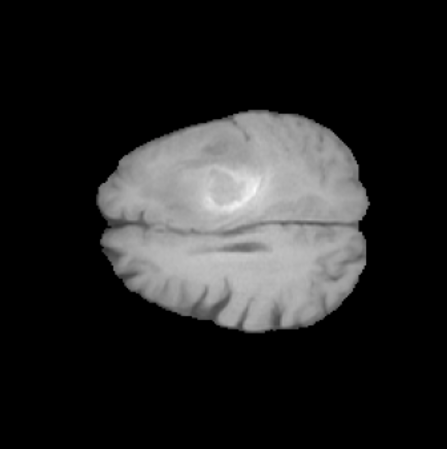
\includegraphics[width=0.4\textwidth]{./Images/Chapter2/t1.png}
        %   \captionsetup{hypcap=false}
        %   \captionof{figure}{Example of T1-weighted MRI sequence.}
        %   \label{fig:t1}
        % \end{minipage}
        % \vspace{\baselineskip}

  \item \textbf{T1 with contrast enhancement (T1ce)}: After gadolinium administration, areas with disrupted blood-brain barrier (characteristic of high-grade tumors) enhance, appearing hyperintense and revealing the active tumor core.

        % \begin{minipage}{\linewidth}
        %   \centering
        %   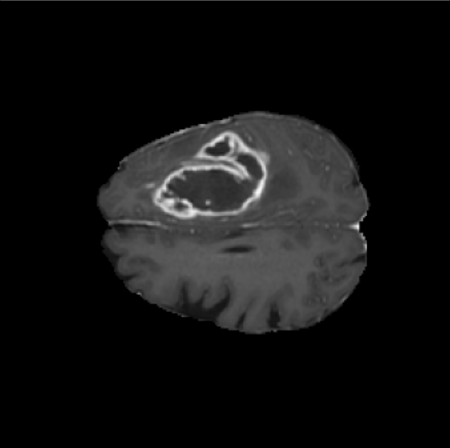
\includegraphics[width=0.4\textwidth]{./Images/Chapter2/t1ce.png}
        %   \captionsetup{hypcap=false}
        %   \captionof{figure}{Example of T1-weighted contrast-enhanced MRI sequence.}
        %   \label{fig:t1ce}
        % \end{minipage}
        % \vspace{\baselineskip}

  \item \textbf{T2-weighted (T2)}: Highlights areas with increased water content, making it valuable for identifying edema and infiltrative tumor components. Tumors and surrounding edema appear hyperintense.

        % \begin{minipage}{\linewidth}
        %   \centering
        %   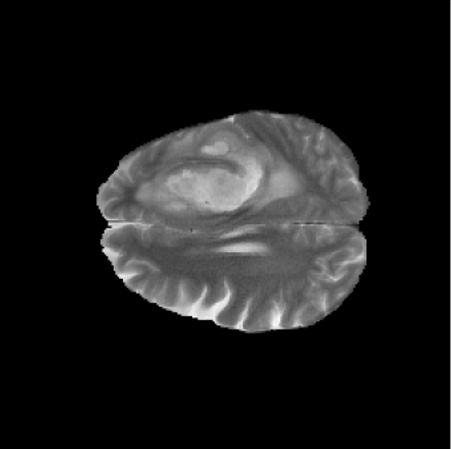
\includegraphics[width=0.4\textwidth]{./Images/Chapter2/t2.png}
        %   \captionsetup{hypcap=false}
        %   \captionof{figure}{Example of T2-weighted MRI sequence.}
        %   \label{fig:t2}
        % \end{minipage}
        % \vspace{\baselineskip}

  \item \textbf{Fluid-Attenuated Inversion Recovery (FLAIR)}: Suppresses cerebrospinal fluid signals, enhancing the visibility of periventricular lesions and edema associated with tumors.

        % \begin{minipage}{\linewidth}
        %   \centering
        %   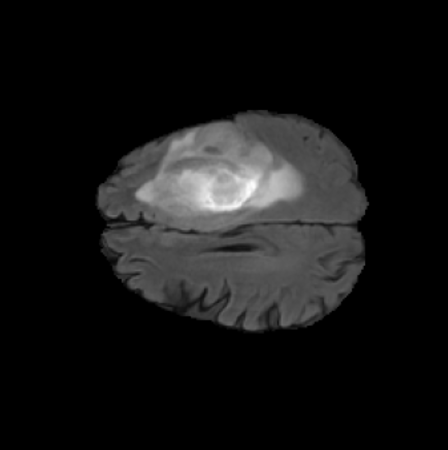
\includegraphics[width=0.4\textwidth]{./Images/Chapter2/flair.png}
        %   \captionsetup{hypcap=false}
        %   \captionof{figure}{Example of FLAIR MRI sequence.}
        %   \label{fig:t2-flair}
        % \end{minipage}
        % \vspace{\baselineskip}
\end{itemize}


Traditionally, neuroradiologists diagnose brain tumors by visually inspecting these multiple MRI sequences, mentally integrating information across modalities to determine tumor boundaries, assess grade, and identify critical structures \cite{DeAngelis2001}. This process is inherently subjective, time-consuming, and susceptible to inter-observer variability, with studies reporting considerable disagreement even among experienced radiologists  These limitations have driven significant interest in developing computational approaches for automated and semi-automated tumor analysis.

\section{Conclusion}
\label{sec:conclusion}

This chapter introduced the fundamental concepts of brain anatomy, tumor classification, and magnetic resonance imaging (MRI) modalities. We discussed the importance of accurate segmentation and classification of brain tumors and the traditional approach of manual diagnosis by radiologists. We also outlined the limitations and challenges of this approach, highlighting the need for computational methods to improve the accuracy and efficiency of brain tumor diagnosis.


